\documentclass[11pt]{article}
\usepackage[utf8]{inputenc}
\usepackage{amsmath, amssymb}
\usepackage{booktabs}
\usepackage{pgfplots}
\pgfplotsset{compat=1.18}
\usepackage{tikz}
\usepackage{xcolor}
\usepackage{geometry}
\geometry{a4paper, margin=1in}
\usepackage{natbib}
\setcitestyle{authoryear, round}

\title{Mathematical Modeling of Hindu Philosophy: Zero, One, and Infinity}
\author{Devendra Soni \\ Independent Researcher \\ \texttt{Erdevendrasoni2022@gmail.com}}
\date{August 17, 2025}

\begin{document}

\maketitle

\begin{abstract}
This paper presents a mathematical framework modeling core Hindu philosophical concepts—Nirguna (formless reality), Saguna (manifest unity), and Anant (infinite consciousness)—through continuous functions, discrete sequences, and limit-based representations. The continuous function \( f(t) = \frac{t}{1+t} \) captures the asymptotic journey from void to unity, the discrete sequence \( A_n \) models hierarchical creation steps, and the limit-based expression unifies zero, one, and infinity. Each model is analyzed with derivations, examples, and visualizations, with tables linking Sanskrit concepts to mathematical constructs and real-world analogies. The framework bridges ancient metaphysics with modern science and has applications in education, AI, and quantum computing.
\end{abstract}

\section{Introduction}
Hindu philosophy, as articulated in texts like the \textit{Upanishads} and \textit{Bhagavad Gita}, conceptualizes the divine through three aspects: Nirguna Brahman (formless reality), Saguna Brahman (manifest unity), and Anant (infinite consciousness). These concepts resonate with mathematical abstractions: zero (0) as the void of origin, one (1) as unity, and infinity (\(\infty\)) as transcendence. This paper formalizes these relationships through mathematical models, offering tools for interdisciplinary research in philosophy, mathematics, physics, and cognitive science.

\section{Literature Review}
The \textit{Chandogya Upanishad} \citep{radhakrishnan1992} describes Brahman as both Nirguna and Saguna, while the \textit{Mandukya Upanishad} \citep{olivelle1998} delineates consciousness states paralleling the 0-to-\(\infty\) transition. The \textit{Bhagavad Gita} \citep{prabhupada1985} balances finite creation with infinite divinity. Ancient Indian mathematicians like Brahmagupta formalized zero and infinity \citep{joseph2000}, providing foundations for symbolic modeling of metaphysical ideas. Modern parallels exist in cosmology \citep{hawking1988}, systems theory \citep{meadows2008}, and quantum physics \citep{despagnat2011}.

\section{Methods and Models}

\subsection{Continuous Model: \( f(t) = \frac{t}{1+t} \)}
\textbf{Definition}: \( f(t) = \frac{t}{1+t} \), \( t \in [0, \infty) \)

\textbf{Mathematical Analysis}:
\begin{itemize}
    \item \(\lim_{t \to 0} f(t) = 0\) (Nirguna) - formless void
    \item \(\lim_{t \to \infty} f(t) = 1\) (Saguna) - manifest unity
    \item \(f'(t) = \frac{1}{(1+t)^2} > 0\) - monotonic growth toward unity
    \item \(f''(t) = -\frac{2}{(1+t)^3} < 0\) - asymptotic slowing
\end{itemize}

% FIXED CONTINUOUS MODEL FIGURE
\begin{figure}[h]
\centering
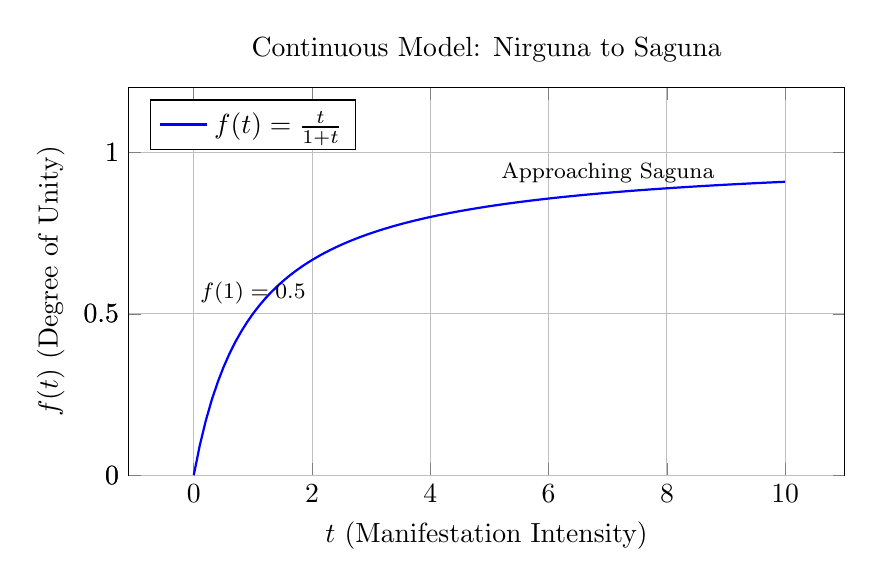
\begin{tikzpicture}
\begin{axis}[
    xlabel={$t$ (Manifestation Intensity)},
    ylabel={$f(t)$ (Degree of Unity)},
    title={Continuous Model: Nirguna to Saguna},
    grid=major,
    domain=0:10,
    samples=100,
    width=0.88\textwidth,
    height=6.5cm,
    ymin=0, ymax=1.2,
    legend pos=north west,
    extra y ticks={0,0.5,1},
    axis background/.style={fill=white},
    xmax=11  % Add extra space on right
]
\addplot[blue, thick] {x/(1+x)};
\addlegendentry{$f(t) = \frac{t}{1+t}$}
\node at (axis cs:0,0) [anchor=north east, font=\footnotesize] {Nirguna (0)};
\node at (axis cs:1,0.5) [anchor=south, font=\footnotesize] {$f(1) = 0.5$};
\node at (axis cs:7,0.875) [anchor=south, font=\footnotesize] {Approaching Saguna}; % Centered position
\end{axis}
\end{tikzpicture}
\caption{Asymptotic progression from formless void to manifest unity}
\label{fig:f_t_plot}
\end{figure}

\begin{table}[h]
\centering
\caption{Continuous Model Values and Interpretation}
\begin{tabular}{c c c c}
\toprule
\( t \) & \( f(t) \) & Interpretation & Sanskrit Concept \\
\midrule
0 & 0.000 & Nirguna: formless void & Nirguna Brahman \\
1 & 0.500 & Initial manifestation & Saguna (early form) \\
2 & 0.667 & Growing complexity & Saguna (expansion) \\
5 & 0.833 & Approaching unity & Saguna (cohesion) \\
10 & 0.909 & Near-perfect unity & Saguna (near-unity) \\
100 & 0.990 & Virtually Saguna & Saguna Brahman \\
\(\infty\) & 1 & Anant: infinite consciousness & Anant \\
\bottomrule
\end{tabular}
\label{tab:continuous}
\end{table}

\subsection{Discrete Model: Creation Ladder}
\textbf{Definition}:
\[
A_n =
\begin{cases}
0, & n = 0 \\
1, & n = 1 \\
2^{n-1}, & n \geq 2
\end{cases}
\]

\textbf{Analysis}:
\begin{itemize}
    \item \(A_0 = 0\): Nirguna (unmanifest void)
    \item \(A_1 = 1\): Saguna (unified reality)
    \item Exponential growth for \(n \geq 2\)
    \item \(\lim_{n \to \infty} A_n = \infty\): Anant (infinite Creator)
    \item Ratio \(\frac{A_{n+1}}{A_n} = 2\): Constant creation momentum
\end{itemize}

\begin{figure}[h]
\centering
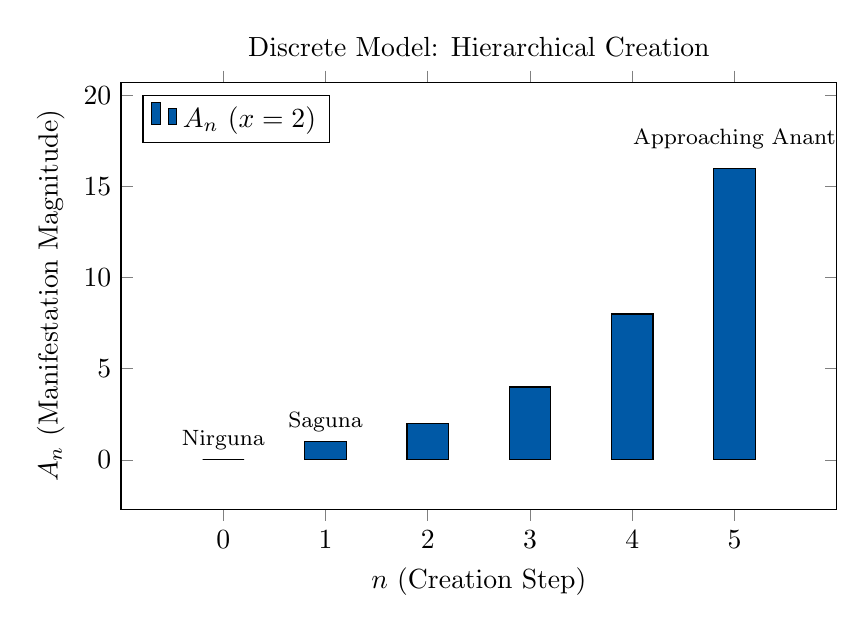
\begin{tikzpicture}
\begin{axis}[
    xlabel={$n$ (Creation Step)},
    ylabel={$A_n$ (Manifestation Magnitude)},
    title={Discrete Model: Hierarchical Creation},
    ybar,
    grid=minor,
    width=0.88\textwidth,
    height=7cm,
    ymin=0, ymax=18,
    xtick={0,1,2,3,4,5},
    bar width=15pt,
    legend pos=north west,
    enlarge x limits=0.2,
    enlarge y limits=0.15
]
\addplot[fill=teal!70!blue] coordinates {(0,0) (1,1) (2,2) (3,4) (4,8) (5,16)};
\addlegendentry{$A_n$ ($x=2$)}
\node at (axis cs:0,0) [anchor=south, font=\footnotesize] {Nirguna};
\node at (axis cs:1,1) [anchor=south, font=\footnotesize] {Saguna};
\node at (axis cs:5,16.5) [anchor=south, font=\footnotesize] {Approaching Anant};
\end{axis}
\end{tikzpicture}
\caption{Discrete emergence from unity to infinite complexity}
\label{fig:A_n_plot}
\end{figure}

\begin{table}[h]
\centering
\caption{Discrete Model Values and Interpretation ($x = 2$)}
\begin{tabular}{c c c c}
\toprule
\( n \) & \( A_n \) & Interpretation & Sanskrit Concept \\
\midrule
0 & 0 & Nirguna: unmanifest void & Nirguna Brahman \\
1 & 1 & Saguna: unified reality & Saguna Brahman \\
2 & 2 & Basic life forms (e.g., cells) & Prajapati (creation) \\
3 & 4 & Ecosystems or interactions & Vishva (cosmic forms) \\
4 & 8 & Complex civilizations & Loka (worlds) \\
5 & 16 & Multi-layered societies & Samsara (cyclic existence) \\
\(\infty\) & \(\infty\) & Anant: infinite Creator & Anant \\
\bottomrule
\end{tabular}
\label{tab:discrete}
\end{table}

\subsection{Limit-Based Model}
\textbf{Definition}: 
\[
\text{God} = \lim_{x \to \infty} (0 + x^n)
\]

\textbf{Mathematical Analysis}:
\begin{itemize}
    \item Unifies Nirguna (0), Saguna (1), and Anant (\(\infty\))
    \item Symbolic representation: \(\text{God} = 0 \cup 1 \cup \infty\)
    \item For fixed \(n\), \(\lim_{x \to \infty} x^n = \infty\)
    \item Captures simultaneous presence of formlessness, unity, and transcendence
\end{itemize}

\section{Combined Framework}
The three models form an integrated representation of Hindu cosmology:
\begin{itemize}
    \item \textbf{Continuous Model}: Seamless evolution from void to unity
    \item \textbf{Discrete Model}: Finite creation steps within infinite framework
    \item \textbf{Limit-Based Model}: Synthesis of 0, 1, \(\infty\) as divine aspects
\end{itemize}

% ORANGE CONCEPTUAL GRAPH
\begin{figure}[h]
\centering
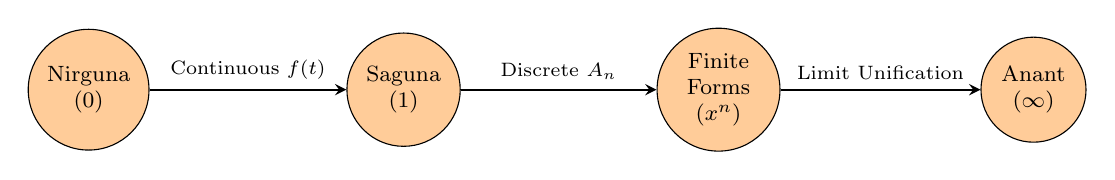
\begin{tikzpicture}[
    node distance=3.8cm,
    node/.style={circle, draw, fill=orange!40, align=center, minimum size=1.3cm, font=\footnotesize}
]
    \node[node] (A) at (0,0) {Nirguna \\ (0)};
    \node[node] (B) at (4,0) {Saguna \\ (1)};
    \node[node] (C) at (8,0) {Finite \\ Forms \\ ($x^n$)};
    \node[node] (D) at (12,0) {Anant \\ ($\infty$)};
    \draw[->, thick, >=stealth] (A) -- (B) node[midway, above, font=\scriptsize] {Continuous $f(t)$};
    \draw[->, thick, >=stealth] (B) -- (C) node[midway, above, font=\scriptsize] {Discrete $A_n$};
    \draw[->, thick, >=stealth] (C) -- (D) node[midway, above, font=\scriptsize] {Limit Unification};
\end{tikzpicture}
\caption{Conceptual integration of philosophical aspects}
\label{fig:conceptual_graph}
\end{figure}

\begin{figure}[h]
\centering
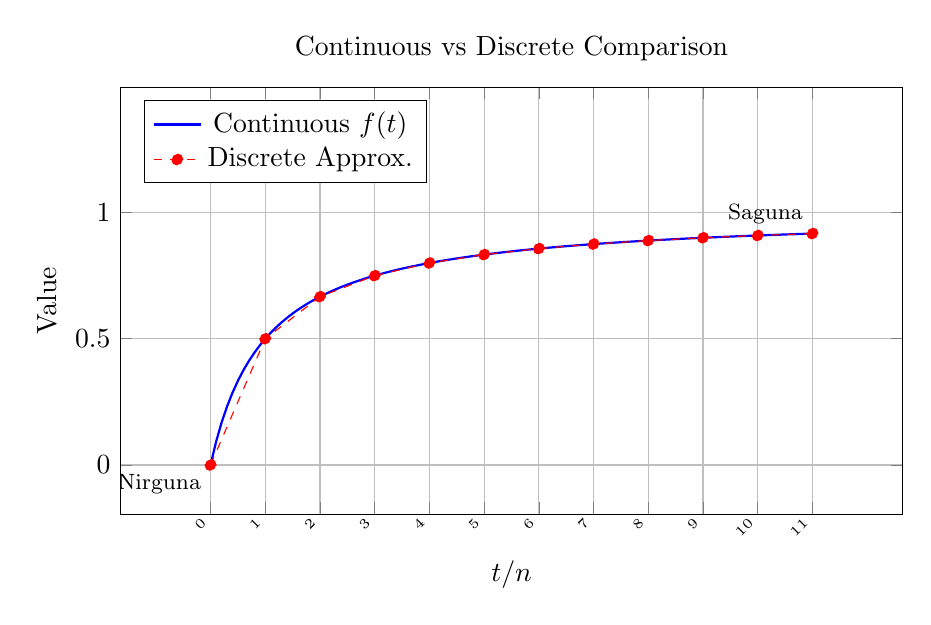
\begin{tikzpicture}
\begin{axis}[
    xlabel={$t/n$},
    ylabel={Value},
    title={Continuous vs Discrete Comparison},
    grid=major,
    width=0.95\textwidth,
    height=7cm,
    ymin=0, ymax=1.3,
    legend pos=north west,
    enlarge x limits=0.15,
    enlarge y limits=0.15,
    xtick={0,1,2,3,4,5,6,7,8,9,10,11},
    xticklabels={0,1,2,3,4,5,6,7,8,9,10,11},
    x tick label style={font=\tiny, rotate=45, anchor=east}
]
\addplot[blue, thick, domain=0:11, samples=110] {x/(1+x)}; 
\addlegendentry{Continuous $f(t)$}
\addplot[red, dashed, mark=*, samples at={0,1,2,3,4,5,6,7,8,9,10,11}] {x/(1+x)};
\addlegendentry{Discrete Approx.}
\node at (axis cs:0,0) [anchor=north east, font=\footnotesize] {Nirguna};
\node at (axis cs:11,0.916) [anchor=south east, font=\footnotesize] {Saguna};
\end{axis}
\end{tikzpicture}
\caption{Continuous and discrete paths to unity}
\label{fig:combined_graph}
\end{figure}

\begin{table}[h]
\centering
\caption{Integrated Mathematical Framework}
\begin{tabular}{l l l l}
\toprule
Model & Mathematical Form & Sanskrit Concept & Real-World Analogy \\
\midrule
Continuous & \( f(t) = \frac{t}{1+t} \) & Nirguna $\to$ Saguna & Quantum vacuum $\to$ unified field \\
Discrete & \( A_n = 2^{n-1} \) & Saguna $\to$ Finite forms & Cosmic structure formation \\
Limit-Based & \( \lim\limits_{x \to \infty} (0 + x^n) \) & 0 $\cup$ 1 $\cup$ $\infty$ & Singularity $\to$ cosmic inflation \\
\bottomrule
\end{tabular}
\label{tab:framework}
\end{table}

\section{Discussion and Implications}

\subsection{Scientific Validations}
\begin{itemize}
    \item \textbf{Quantum Physics}: Nirguna (0) parallels quantum vacuum fluctuations \citep{despagnat2011}
    \item \textbf{Cosmology}: Saguna (1) mirrors symmetry breaking post-Big Bang \citep{hawking1988}
    \item \textbf{Cognitive Science}: Continuous model reflects meditative progression \citep{kabatzinn2013}
    \item \textbf{Systems Theory}: Discrete model aligns with hierarchical emergence \citep{meadows2008}
\end{itemize}

\subsection{Applications}
\textbf{Education}:
\begin{itemize}
    \item Visualizing metaphysical concepts through mathematical plots
    \item Teaching limits through philosophical analogies
\end{itemize}

\textbf{Technology}:
\begin{itemize}
    \item AI consciousness: Nirguna as latent space, Saguna as algorithms, Anant as emergent intelligence
    \item Quantum computing: Qubit entanglement as infinity-from-unity principle
\end{itemize}

\textbf{Cross-Cultural Dialogue}: Universal symbolic language for comparative metaphysics

\subsection{Limitations}
\begin{itemize}
    \item Symbolic rather than empirical framework
    \item Requires basic calculus knowledge
    \item Interpretations vary across Hindu traditions
\end{itemize}

\section{Conclusion}
This work establishes a mathematical framework for Hindu philosophical concepts, integrating continuous, discrete, and limit-based models. By formalizing Nirguna (0), Saguna (1), and Anant (\(\infty\)), it bridges ancient Vedanta with modern science. Future directions include modeling cyclic time (Yugas) and extending the framework to other philosophical traditions.

\begin{thebibliography}{9}
\bibitem[Berndt, 1994]{berndt1994} Berndt, B. C. (1994). \textit{Ramanujan's Notebooks: Part IV}. Springer.
\bibitem[D'Espagnat, 2011]{despagnat2011} D'Espagnat, B. (2011). Quantum physics and Vedanta. \textit{Zygon}, 46(3), 620-631.
\bibitem[Duquette, 2011]{duquette2011} Duquette, J. (2011). Quantum physics and Vedanta. \textit{Zygon}, 46(3), 620-638.
\bibitem[Hawking, 1988]{hawking1988} Hawking, S. W. (1988). \textit{A Brief History of Time}. Bantam.
\bibitem[Joseph, 2000]{joseph2000} Joseph, G. G. (2000). \textit{The Crest of the Peacock}. Princeton.
\bibitem[Kabat-Zinn, 2013]{kabatzinn2013} Kabat-Zinn, J. (2013). \textit{Full Catastrophe Living}. Bantam.
\bibitem[Meadows, 2008]{meadows2008} Meadows, D. H. (2008). \textit{Thinking in Systems}. Chelsea Green.
\bibitem[Olivelle, 1998]{olivelle1998} Olivelle, P. (1998). \textit{The Early Upanishads}. Oxford.
\bibitem[Prabhupada, 1985]{prabhupada1985} Prabhupada, A. C. B. S. (1985). \textit{Bhagavad-Gita As It Is}. Bhaktivedanta.
\bibitem[Radhakrishnan, 1992]{radhakrishnan1992} Radhakrishnan, S. (1992). \textit{The Principal Upanishads}. HarperCollins.
\end{thebibliography}

\end{document}